% answers.tex —— 2010 年·普通高等学校招生考试·湖南卷·理科 · 参考答案与详细解析片段
% 由 tools/generate_projects.py 依来源总账自 2010/2010_数学真题_湖南理_试题.md + 2010/2010_数学真题_湖南理_解析正文.md + 2010/2010_数学真题_湖南理_答案要点.md 生成，勿手改（改源 MD 后重跑）
\begin{gktip}
固定候选 PDF 仅含题面、无答案页；以下解析与结论均由本库独立推导（非官方答案），并按 600 dpi 原页复核题面。原页未印分值，不补。
\end{gktip}

\begin{answer}
\gksolhead{1}{}

\textbf{题目}：

已知集合 $M=\{1,2,3\}$，$N=\{2,3,4\}$，则（　）

（A）$M\subseteq N$

（B）$N\subseteq M$

（C）$M\cap N=\{2,3\}$

（D）$M\cup N=\{1,4\}$

\Needspace{4\baselineskip}
\textbf{解析}
\Needspace{5\baselineskip}
$M=\{1,2,3\}$，$N=\{2,3,4\}$，故
\nopagebreak[4]
\[M\cap N=\{2,3\},\qquad M\cup N=\{1,2,3,4\}.\]
逐项排除：$1\in M$ 而 $1\notin N$，故 $M\not\subseteq N$，A 错；$4\in N$ 而 $4\notin M$，故 $N\not\subseteq M$，B 错；$M\cup N=\{1,2,3,4\}\neq\{1,4\}$，D 错。C 正确。
故选 C。

\gkanswer{答案：C。}

\end{answer}
\begin{answer}
\gksolhead{2}{}

\textbf{题目}：

下列命题中是假命题的是（　）

（A）$\forall x\in\mathbf R$，$2^{x-1}>0$

（B）$\forall x\in\mathbf N^*$，$(x-1)^2>0$

（C）$\exists x\in\mathbf R$，$\lg x<1$

（D）$\exists x\in\mathbf R$，$\tan x=2$

\Needspace{4\baselineskip}
\textbf{解析}
A：指数函数 $2^{x-1}>0$ 对一切实数 $x$ 成立，是真命题。
B：取 $x=1\in\mathbf N^*$，则 $(x-1)^2=0$，不满足 $>0$，是假命题。
C：取 $x=1$，$\lg1=0<1$，是真命题。
D：$\tan x$ 的值域为 $\mathbf R$，故存在 $x\in\mathbf R$ 使 $\tan x=2$，是真命题。
故选 B。

\gkanswer{答案：B。}

\end{answer}
\begin{answer}
\gksolhead{3}{}

\textbf{题目}：

极坐标方程 $\rho=\cos\theta$ 和参数方程 $\begin{cases}x=-1-t,\\ y=2+3t\end{cases}$（$t$ 为参数）所表示的图形分别是（　）

（A）圆、直线

（B）直线、圆

（C）圆、圆

（D）直线、直线

\Needspace{4\baselineskip}
\textbf{解析}
\Needspace{5\baselineskip}
由 $\rho=\cos\theta$ 得 $\rho^2=\rho\cos\theta$，即
\nopagebreak[4]
\[x^2+y^2=x\iff\left(x-\frac12\right)^2+y^2=\frac14,\]
表示圆。
\Needspace{5\baselineskip}
参数方程中由 $x=-1-t$ 得 $t=-1-x$，代入 $y=2+3t$：
\nopagebreak[4]
\[y=2+3(-1-x)=-3x-1,\]
即 $3x+y+1=0$，表示直线。
故前者为圆、后者为直线。
故选 A。

\gkanswer{答案：A。}

\end{answer}
\begin{answer}
\gksolhead{4}{}

\textbf{题目}：

在 $\mathrm{Rt}\triangle ABC$ 中，$\angle C=90^\circ$，$AC=4$，则 $\overrightarrow{AB}\cdot\overrightarrow{AC}$ 等于（　）

（A）$-16$

（B）$-8$

（C）$8$

（D）$16$

\Needspace{4\baselineskip}
\textbf{解析}
\Needspace{5\baselineskip}
在 $\mathrm{Rt}\triangle ABC$ 中 $\angle C=90^\circ$，故 $\overrightarrow{AB}$ 在 $\overrightarrow{AC}$ 方向上的投影为 $|\overrightarrow{AC}|$。于是
\nopagebreak[4]
\[\overrightarrow{AB}\cdot\overrightarrow{AC}=|\overrightarrow{AB}|\cdot|\overrightarrow{AC}|\cos\angle BAC
=|\overrightarrow{AC}|\cdot\bigl(|\overrightarrow{AB}|\cos\angle BAC\bigr)
=|\overrightarrow{AC}|^2=16.\]
故选 D。

\gkanswer{答案：D。}

\end{answer}
\begin{answer}
\gksolhead{5}{}

\textbf{题目}：

$\displaystyle\int_2^4\frac1x\,\mathrm dx$ 等于（　）

（A）$-2\ln2$

（B）$2\ln2$

（C）$-\ln2$

（D）$\ln2$

\Needspace{4\baselineskip}
\textbf{解析}
\nopagebreak[4]
\[\int_2^4\frac1x\,\mathrm dx=\bigl[\ln x\bigr]_2^4=\ln4-\ln2=\ln2.\]
故选 D。

\gkanswer{答案：D。}

\end{answer}
\begin{answer}
\gksolhead{6}{}

\textbf{题目}：

在 $\triangle ABC$ 中，角 $A$，$B$，$C$ 所对的边长分别为 $a$，$b$，$c$，若 $\angle C=120^\circ$，$c=\sqrt2a$，则（　）

（A）$a>b$

（B）$a<b$

（C）$a=b$

（D）$a$ 与 $b$ 的大小关系不能确定

\Needspace{4\baselineskip}
\textbf{解析}
\Needspace{5\baselineskip}
由余弦定理，$\angle C=120^\circ$ 时
\nopagebreak[4]
\[c^2=a^2+b^2-2ab\cos120^\circ=a^2+b^2+ab.\]
\Needspace{5\baselineskip}
又 $c^2=2a^2$，故
\nopagebreak[4]
\[2a^2=a^2+b^2+ab\iff a^2-ab-b^2=0.\]
\Needspace{5\baselineskip}
两边除以 $b^2>0$，令 $t=\dfrac ab>0$，得 $t^2-t-1=0$，故
\nopagebreak[4]
\[t=\frac{1+\sqrt5}{2}>1\iff a>b.\]
故选 A。

\gkanswer{答案：A。}

\end{answer}
\begin{answer}
\gksolhead{7}{}

\textbf{题目}：

在某种信息传输过程中，用 $4$ 个数字的一个排列（数字允许重复）表示一个信息，不同排列表示不同信息，若所用数字只有 $0$ 和 $1$，则与信息 $0110$ 至多有两个对应位置上的数字相同的信息个数为（　）

（A）$10$

（B）$11$

（C）$12$

（D）$15$

\Needspace{4\baselineskip}
\textbf{解析}
\Needspace{5\baselineskip}
用 $0$、$1$ 组成的 $4$ 位信息共 $2^4=16$ 个。与 $0110$ 有 $4$ 个对应位置数字相同的信息只有 $0110$ 本身，共 $1$ 个；有 $3$ 个位置相同即恰有一个位置不同（把某一位 $0$ 改 $1$ 或 $1$ 改 $0$），共 $4$ 个。故“至多有两个位置相同”的信息数为
\nopagebreak[4]
\[16-1-4=11.\]
故选 B。

\gkanswer{答案：B。}

\end{answer}
\begin{answer}
\gksolhead{8}{}

\textbf{题目}：

用 $\min\{a,b\}$ 表示 $a$，$b$ 两数中的最小值。若函数 $f(x)=\min\{|x|,|x+t|\}$ 的图象关于直线 $x=-\dfrac12$ 对称，则 $t$ 的值为（　）

（A）$-2$

（B）$2$

（C）$-1$

（D）$1$

\Needspace{4\baselineskip}
\textbf{解析}
\Needspace{5\baselineskip}
$|x|$ 的图象关于直线 $x=0$ 对称，$|x+t|$ 的图象关于直线 $x=-t$ 对称。关于两对称轴的中点作反射，会把其中一个函数变为另一个，故 $f(x)=\min\{|x|,|x+t|\}$ 的图象关于直线
\nopagebreak[4]
\[x=\frac{0+(-t)}2=-\frac t2\]
\Needspace{5\baselineskip}
对称。由题设 $-\dfrac t2=-\dfrac12$，得
\nopagebreak[4]
\[t=1.\]
检验：$t=1$ 时 $f(x)=\min\{|x|,|x+1|\}$，关于 $x=-\dfrac12$ 对称，符合。
故选 D。

\gkanswer{答案：D。}

\end{answer}
\begin{answer}
\gksolhead{9}{}

\textbf{题目}：

已知一种材料的最佳加入量在 $110$ g 到 $210$ g 之间。若用 $0.618$ 法安排实验，则第一次试点的加入量可以是 $\underline{\qquad}$ g。

\Needspace{4\baselineskip}
\textbf{解析}
\Needspace{5\baselineskip}
区间长度为 $210-110=100$ g。按 $0.618$ 法，第一个试点可取
\nopagebreak[4]
\[110+0.618\times100=171.8,\]
\Needspace{5\baselineskip}
或从另一端取
\nopagebreak[4]
\[210-0.618\times100=148.2.\]
两者都是“可以”的第一次试点加入量（单位：g）。
故填 $171.8$ 或 $148.2$。

\gkanswer{答案：$171.8$ g 或 $148.2$ g。}

\end{answer}
\begin{answer}
\gksolhead{10}{}

\textbf{题目}：

如图所示，过 $\odot O$ 外一点 $P$ 作一条直线与 $\odot O$ 交于 $A$，$B$ 两点。已知 $PA=2$，点 $P$ 到 $\odot O$ 的切线长 $PT=4$，则弦 $AB$ 的长为 $\underline{\qquad}$。
\nopagebreak[4]
\begin{center}% 2010 年湖南卷理科第 10 题：⊙O 外一点 P 的切线与割线。
% 来源 PDF：普通高考/2010/2010湖南理.pdf，SHA-256 db6274a80ebb0022ff1b91b2cd3714fe8cca335e48be69805dcd87cdefd8c8d1。
% 原页：第 1 页（A3 三栏）第 2 栏上部，书页码 601。
% 重绘依据：照原页，圆心 O 在圆内偏右上；P 在圆外左下，PT 为切线（T 在圆左上），
%   割线自 P 向右穿过圆于 A（近 P）与 B（远 P），A、B 在圆上，弦 AB 近似水平。
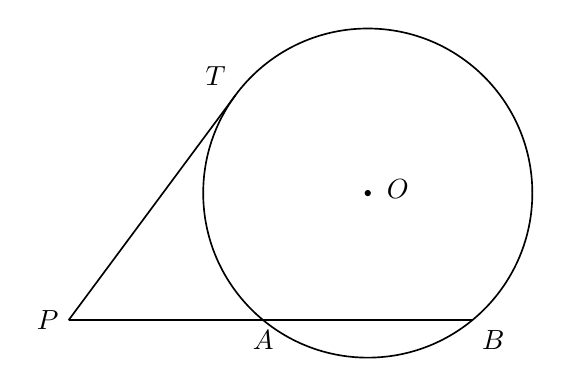
\begin{tikzpicture}[scale=0.95, semithick]
  \coordinate (O) at (0,0);
  \coordinate (P) at (-4,-1.7);
  \coordinate (T) at (-1.767,1.31);
  \coordinate (A) at (-1.396,-1.7);
  \coordinate (B) at (1.396,-1.7);

  \draw (O) circle (2.2);
  \fill (O) circle (1.2pt);
  \node[right] at (0.12,0.06) {$O$};

  \draw (P) -- (T);
  \draw (P) -- (B);

  \node[above left] at (T) {$T$};
  \node[left] at (P) {$P$};
  \node[below] at (A) {$A$};
  \node[below right] at (B) {$B$};
\end{tikzpicture}
\end{center}
\nopagebreak[4]
\Needspace{4\baselineskip}
\textbf{解析}
\Needspace{5\baselineskip}
由切割线定理，
\nopagebreak[4]
\[PT^2=PA\cdot PB.\]
\Needspace{5\baselineskip}
代入 $PT=4$，$PA=2$：
\nopagebreak[4]
\[16=2\cdot PB\iff PB=8,\]
\Needspace{5\baselineskip}
故
\nopagebreak[4]
\[AB=PB-PA=8-2=6.\]
检验：$PA\cdot PB=2\times8=16=PT^2$，符合。
故填 $6$。

\gkanswer{答案：$6$。}

\end{answer}
\begin{answer}
\gksolhead{11}{}

\textbf{题目}：

在区间 $[-1,2]$ 上随机取一个数 $x$，则 $|x|\leqslant1$ 的概率为 $\underline{\qquad}$。

\Needspace{4\baselineskip}
\textbf{解析}
\Needspace{5\baselineskip}
区间 $[-1,2]$ 的长度为 $3$。条件 $|x|\leqslant1$ 即 $-1\leqslant x\leqslant1$，它与 $[-1,2]$ 的交集为 $[-1,1]$，长度为 $2$。故所求概率为
\nopagebreak[4]
\[\frac{2}{3}.\]
故填 $\dfrac23$。

\gkanswer{答案：$\dfrac23$。}

\end{answer}
\begin{answer}
\gksolhead{12}{}

\textbf{题目}：

如图是求 $1^2+2^2+3^2+\cdots+100^2$ 的值的程序框图，则正整数 $n=$ $\underline{\qquad}$。
\nopagebreak[4]
\begin{center}% 2010 年湖南卷理科第 12 题：求 1^2+2^2+...+100^2 的程序框图。
% 来源 PDF：普通高考/2010/2010湖南理.pdf，SHA-256 db6274a80ebb0022ff1b91b2cd3714fe8cca335e48be69805dcd87cdefd8c8d1。
% 原页：第 1 页（A3 三栏）第 2 栏中部，书页码 601。
% 重绘依据：照原页，开始→i=1,s=0→判断 i<=n?；判断框「是」向右、向上依次经
%   s=s+i^2、i=i+1 后向左汇入主干（即在判断前先累加再自增）；「否」向下经输出 s 到结束。
\begin{tikzpicture}[scale=1.0, semithick,
  every node/.style={inner sep=2pt},
  box/.style={draw, minimum width=2.6cm, minimum height=0.6cm, align=center},
  round/.style={draw, rounded corners=6pt, minimum width=1.5cm,
    minimum height=0.6cm, align=center},
  para/.style={draw, trapezium, trapezium left angle=70, trapezium right angle=110,
    minimum width=2.2cm, minimum height=0.65cm, align=center},
  dec/.style={draw, diamond, aspect=2.4, minimum width=2.8cm,
    minimum height=1.1cm, align=center},
  arr/.style={->, >=stealth}]

  \node[round] (start) at (0,9.1) {开始};
  \node[box]   (init)  at (0,8.1) {$i=1,\ s=0$};
  \node[dec]   (test)  at (0,4.9) {$i\leqslant n$?};
  \node[para]  (out)   at (0,3.0) {输出 $s$};
  \node[round] (end)   at (0,1.9) {结束};

  \node[box] (sum) at (3.5,5.9) {$s=s+i^2$};
  \node[box] (inc) at (3.5,7.2) {$i=i+1$};

  \draw[arr] (start) -- (init);
  \draw[arr] (init) -- (test);
  \draw[arr] (test.south) -- (out.north);
  \node[right] at (0.14,3.85) {否};
  \draw[arr] (out) -- (end);

  \draw[arr] (test.east) -| (sum.south);
  \node[right] at (1.75,5.08) {是};
  \draw[arr] (sum.north) -- (inc.south);
  \draw[arr] (inc.west) -- (0,7.2);
\end{tikzpicture}
\end{center}
\nopagebreak[4]
\Needspace{4\baselineskip}
\textbf{解析}
按框图模拟：初值 $i=1$，$s=0$；循环体内先算 $s=s+i^2$，再算 $i=i+1$，然后判断 $i\leqslant n$，成立则返回循环，否则输出 $s$。
\Needspace{5\baselineskip}
因此循环依次把 $i=1,2,\cdots,n$ 的平方累加，输出
\nopagebreak[4]
\[s=1^2+2^2+\cdots+n^2.\]
\Needspace{5\baselineskip}
题设要求输出 $1^2+2^2+\cdots+100^2$，故
\nopagebreak[4]
\[n=100.\]
检验：$n=99$ 时只累加到 $99^2$，$n=101$ 时会多算 $101^2$，均不合。
故填 $100$。

\gkanswer{答案：$100$。}

\end{answer}
\begin{answer}
\gksolhead{13}{}

\textbf{题目}：

图中的三个直角三角形是一个体积为 $20$ cm$^3$ 的几何体的三视图，则 $h=$ $\underline{\qquad}$ cm。
\nopagebreak[4]
\begin{center}% 2010 年湖南卷理科第 13 题：体积 20 cm^3 的几何体的三视图。
% 来源 PDF：普通高考/2010/2010湖南理.pdf，SHA-256 db6274a80ebb0022ff1b91b2cd3714fe8cca335e48be69805dcd87cdefd8c8d1。
% 原页：第 1 页（A3 三栏）第 2 栏下部，书页码 601。
% 重绘依据：三个直角三角形——正视图直角边 5 与 h（直角在左下），
%   侧视图直角边 6 与 h（直角在左下），俯视图直角边 5、6（直角在左上）；
%   俯视图在原页未标数字，此处亦不标。图中 h 按原页比例虚设，不代表答案。
\begin{tikzpicture}[scale=0.62, semithick]
  % 正视图：宽 5，高 h
  \draw (0,0) -- (5,0) -- (0,3.2) -- cycle;
  \draw[<->] (-0.6,0) -- (-0.6,3.2);
  \draw (-0.75,0) -- (-0.35,0);
  \draw (-0.75,3.2) -- (-0.35,3.2);
  \node[left] at (-0.85,1.6) {$h$};
  \draw[<->] (0,-0.6) -- (5,-0.6);
  \draw (0,-0.75) -- (0,-0.35);
  \draw (5,-0.75) -- (5,-0.35);
  \node[below] at (2.5,-0.55) {$5$};
  \node[below] at (2.5,-1.45) {正视图};

  % 侧视图：宽 6，高 h
  \draw (7.6,0) -- (13.6,0) -- (7.6,3.2) -- cycle;
  \draw[<->] (7.6,-0.6) -- (13.6,-0.6);
  \draw (7.6,-0.75) -- (7.6,-0.35);
  \draw (13.6,-0.75) -- (13.6,-0.35);
  \node[below] at (10.6,-0.55) {$6$};
  \node[below] at (10.6,-1.45) {侧视图};

  % 俯视图：宽 5，高 6，直角在左上
  \draw (0,-4.6) -- (5,-4.6) -- (0,-10.6) -- cycle;
  \node[below] at (2.5,-10.9) {俯视图};
\end{tikzpicture}
\end{center}
\nopagebreak[4]
\Needspace{4\baselineskip}
\textbf{解析}
由三视图：正视图是直角边长 $5$、$h$ 的直角三角形，侧视图是直角边长 $6$、$h$ 的直角三角形，俯视图是直角边长 $5$、$6$ 的直角三角形。故该几何体是一个三棱锥，从同一顶点出发的三条棱两两垂直，长度分别为 $5$、$6$、$h$。
\Needspace{5\baselineskip}
以这三条棱为棱，体积为
\nopagebreak[4]
\[V=\frac16\cdot5\cdot6\cdot h=5h.\]
\Needspace{5\baselineskip}
由 $V=20$ 得
\nopagebreak[4]
\[5h=20\iff h=4.\]
检验：$\dfrac16\times5\times6\times4=20$，符合。
故填 $4$。

\gkanswer{答案：$4$。}

\end{answer}
\begin{answer}
\gksolhead{14}{}

\textbf{题目}：

过抛物线 $x^2=2py$（$p>0$）的焦点作斜率为 $1$ 的直线与该抛物线交于 $A$，$B$ 两点，$A$，$B$ 在 $x$ 轴上的正射影分别为 $D$，$C$。若梯形 $ABCD$ 的面积为 $12\sqrt2$，则 $p=$ $\underline{\qquad}$。

\Needspace{4\baselineskip}
\textbf{解析}
\Needspace{5\baselineskip}
抛物线 $x^2=2py$ 的焦点为 $F\left(0,\dfrac p2\right)$，斜率为 $1$ 的直线为
\nopagebreak[4]
\[y=x+\frac p2.\]
\Needspace{5\baselineskip}
代入 $x^2=2py$：
\nopagebreak[4]
\[x^2=2p\left(x+\frac p2\right)\iff x^2-2px-p^2=0.\]
\Needspace{5\baselineskip}
设 $A(x_1,y_1)$，$B(x_2,y_2)$，则
\nopagebreak[4]
\[x_1+x_2=2p,\qquad x_1x_2=-p^2,\qquad |x_1-x_2|=\sqrt{(2p)^2+4p^2}=2\sqrt2\,p.\]
\Needspace{5\baselineskip}
又 $y_1=x_1+\dfrac p2$，$y_2=x_2+\dfrac p2$，故
\nopagebreak[4]
\[y_1+y_2=x_1+x_2+p=3p.\]
\Needspace{5\baselineskip}
梯形 $ABCD$ 中 $AD$、$BC$ 都垂直于 $x$ 轴，$AD=y_1$，$BC=y_2$，$DC=|x_1-x_2|$，故
\nopagebreak[4]
\[S=\frac12(y_1+y_2)\,|x_1-x_2|=\frac12\cdot3p\cdot2\sqrt2\,p=3\sqrt2\,p^2.\]
\Needspace{5\baselineskip}
由 $3\sqrt2\,p^2=12\sqrt2$ 得 $p^2=4$，又 $p>0$，故
\nopagebreak[4]
\[p=2.\]
检验：$p=2$ 时 $S=3\sqrt2\times4=12\sqrt2$，符合。
故填 $2$。

\gkanswer{答案：$2$。}

\end{answer}
\begin{answer}
\gksolhead{15}{}

\textbf{题目}：

若数列 $\{a_n\}$ 满足：对任意的 $n\in\mathbf N^*$，只有有限个正整数 $m$ 使得 $a_m<n$ 成立，记这样的 $m$ 的个数为 $(a_n)^*$，则得到一个新数列 $\{(a_n)^*\}$。例如，若数列 $\{a_n\}$ 是 $1,2,3,\cdots,n,\cdots$，则数列 $\{(a_n)^*\}$ 是 $0,1,2,\cdots,n-1,\cdots$。已知对任意的 $n\in\mathbf N^*$，$a_n=n^2$，则 $(a_5)^*=$ $\underline{\qquad}$，$((a_n)^*)^*=$ $\underline{\qquad}$。

\Needspace{4\baselineskip}
\textbf{解析}
\Needspace{5\baselineskip}
当 $a_n=n^2$ 时，$a_m<n\iff m^2<n\iff m\leqslant\lfloor\sqrt{n-1}\rfloor$。故 $(a_n)^*$ 是满足 $m^2<n$ 的正整数 $m$ 的个数，即
\nopagebreak[4]
\[(a_n)^*=\bigl\lfloor\sqrt{n-1}\bigr\rfloor.\]
\Needspace{5\baselineskip}
取 $n=5$：$m^2<5$ 给出 $m=1,2$，故
\nopagebreak[4]
\[(a_5)^*=2.\]
\Needspace{5\baselineskip}
记 $b_n=(a_n)^*=\lfloor\sqrt{n-1}\rfloor$。则 $((a_n)^*)^*$ 是满足 $b_m<n$ 的正整数 $m$ 的个数。由
\nopagebreak[4]
\[b_m<n\iff\bigl\lfloor\sqrt{m-1}\bigr\rfloor\leqslant n-1\iff\sqrt{m-1}<n\iff m<n^2+1,\]
\Needspace{5\baselineskip}
得 $m=1,2,\cdots,n^2$，共 $n^2$ 个，故
\nopagebreak[4]
\[((a_n)^*)^*=n^2.\]
检验：$n=5$ 时 $b_m<5$ 即 $\lfloor\sqrt{m-1}\rfloor\leqslant4$，得 $m\leqslant25$，共 $25=5^2$ 个，符合。
故填 $2$，$n^2$。

\gkanswer{答案：$2$；$n^2$。}

\end{answer}
\begin{answer}
\gksolhead{16}{}

\textbf{题目}：

已知函数 $f(x)=\sqrt3\sin2x-2\sin^2x$。

（1）求函数 $f(x)$ 的最大值；

（2）求函数 $f(x)$ 的零点的集合。

\Needspace{4\baselineskip}
\textbf{解析}
\Needspace{5\baselineskip}
（1）
\nopagebreak[4]
\[f(x)=\sqrt3\sin2x-2\sin^2x=\sqrt3\sin2x+\cos2x-1
=2\sin\left(2x+\frac\pi6\right)-1.\]
\Needspace{5\baselineskip}
故当 $\sin\left(2x+\dfrac\pi6\right)=1$ 时 $f(x)$ 取最大值
\nopagebreak[4]
\[f_{\max}=2-1=1.\]
\Needspace{5\baselineskip}
（2）令 $f(x)=0$：
\nopagebreak[4]
\[2\sin\left(2x+\frac\pi6\right)-1=0\iff\sin\left(2x+\frac\pi6\right)=\frac12.\]
\Needspace{5\baselineskip}
于是
\nopagebreak[4]
\[2x+\frac\pi6=\frac\pi6+2k\pi\quad\text{\text{或}}\quad2x+\frac\pi6=\frac{5\pi}6+2k\pi\quad(k\in\mathbf Z),\]
\Needspace{5\baselineskip}
即
\nopagebreak[4]
\[x=k\pi\quad\text{\text{或}}\quad x=\frac\pi3+k\pi\quad(k\in\mathbf Z).\]
\Needspace{5\baselineskip}
故零点的集合为
\nopagebreak[4]
\[\left\{x\ \middle|\ x=k\pi\ \text{\text{或}}\ x=k\pi+\frac\pi3,\ k\in\mathbf Z\right\}.\]

\gkanswer{答案：（1）$1$；（2）$\left\{x\ \middle|\ x=k\pi\ \text{\text{或}}\ x=k\pi+\dfrac\pi3,\ k\in\mathbf Z\right\}$。}

\end{answer}
\begin{answer}
\gksolhead{17}{}

\textbf{题目}：

如图，是某城市通过抽样得到的居民某年的月均用水量（单位：吨）的频率分布直方图。

（1）求直方图中 $x$ 的值；

（2）若将频率视为概率，从这个城市随机抽取 $3$ 位居民（看作有放回的抽样），求月均用水量在 $3$ 至 $4$ 吨的居民数 $X$ 的分布列和数学期望。
\nopagebreak[4]
\begin{center}% 2010 年湖南卷理科第 17 题：月均用水量的频率分布直方图。
% 来源 PDF：普通高考/2010/2010湖南理.pdf，SHA-256 db6274a80ebb0022ff1b91b2cd3714fe8cca335e48be69805dcd87cdefd8c8d1。
% 原页：第 1 页（A3 三栏）第 3 栏中部，书页码 601。
% 重绘依据：组距 1，五组 [0,1]、[1,2]、[2,3]、[3,4]、[4,5] 的高度依次为
%   x、0.37、0.39、0.1、0.02；纵轴标「频率/组距」，横轴标「月均用水量/吨」；
%   0.39、0.37、0.1、0.02 以虚线引到对应矩形条顶部。
\begin{tikzpicture}[x=1.2cm, y=10cm, semithick, font=\scriptsize]
  \draw[->] (0,0) -- (8.4,0);
  \draw[->] (0,0) -- (0,0.55);
  \node[anchor=west, font=\small] at (0.04,0.535) {频率};
  \node[anchor=west, font=\small] at (0.04,0.492) {组距};

  % 五个矩形条（组距 1）
  \draw (0,0) rectangle (1,0.12);
  \draw (1,0) rectangle (2,0.37);
  \draw (2,0) rectangle (3,0.39);
  \draw (3,0) rectangle (4,0.10);
  \draw (4,0) rectangle (5,0.02);

  % 横轴刻度
  \foreach \k in {0,1,2,3,4,5} {
    \draw (\k,0) -- ++(0,-0.008);
    \node[below] at (\k,-0.010) {\k};
  }
  \node[anchor=west, font=\small] at (5.35,-0.012) {月均用水量/吨};

  % 纵轴读数与虚线
  \draw[dashed] (0,0.39) -- (2,0.39);
  \draw[dashed] (0,0.37) -- (1,0.37);
  \draw[dashed] (0,0.10) -- (3,0.10);
  \draw[dashed] (0,0.02) -- (4,0.02);
  \node[left] at (0,0.405) {0.39};
  \node[left] at (0,0.37) {0.37};
  \node[left] at (0,0.12) {$x$};
  \node[left] at (0,0.10) {0.1};
  \node[left] at (0,0.02) {0.02};
\end{tikzpicture}
\end{center}
\nopagebreak[4]
\Needspace{4\baselineskip}
\textbf{解析}
\Needspace{5\baselineskip}
（1）各矩形条面积之和为 $1$，组距为 $1$，故
\nopagebreak[4]
\[x+0.37+0.39+0.1+0.02=1\iff x=0.12.\]
\Needspace{5\baselineskip}
（2）月均用水量在 $3$ 至 $4$ 吨的频率为 $0.1$，视为概率，故每位居民落在该组的概率 $p=0.1$，且
\nopagebreak[4]
\[X\sim B(3,0.1).\]
\Needspace{5\baselineskip}
于是
\nopagebreak[4]
\[P(X=k)=\mathrm C_3^k(0.1)^k(0.9)^{3-k},\qquad k=0,1,2,3.\]
\Needspace{5\baselineskip}
分布列为
\nopagebreak[4]
\[\begin{array}{c|cccc}
X & 0 & 1 & 2 & 3\\ \hline
P & 0.729 & 0.243 & 0.027 & 0.001
\end{array}\]
\Needspace{5\baselineskip}
数学期望
\nopagebreak[4]
\[EX=3\times0.1=0.3.\]
检验：$0.729+0.243+0.027+0.001=1$，符合。

\gkanswer{答案：（1）$0.12$；（2）$P(X=0)=0.729$，$P(X=1)=0.243$，$P(X=2)=0.027$，$P(X=3)=0.001$，$EX=0.3$。}

\end{answer}
\begin{answer}
\gksolhead{18}{}

\textbf{题目}：

如图所示，在正方体 $ABCD-A_1B_1C_1D_1$ 中，$E$ 是棱 $DD_1$ 的中点。

（1）求直线 $BE$ 和平面 $ABB_1A_1$ 所成的角的正弦值；

（2）在棱 $C_1D_1$ 上是否存在一点 $F$，使 $B_1F\parallel$ 平面 $A_1BE$？证明你的结论。
\nopagebreak[4]
\begin{center}% 2010 年湖南卷理科第 18 题：正方体 ABCD-A1B1C1D1，E 为棱 DD1 的中点。
% 来源 PDF：普通高考/2010/2010湖南理.pdf，SHA-256 db6274a80ebb0022ff1b91b2cd3714fe8cca335e48be69805dcd87cdefd8c8d1。
% 原页：第 2 页（A3 三栏）第 1 栏上部，书页码 602。
% 重绘依据：照原页斜二测画法，前面 BB1C1C，后面 AA1D1D 向右上平移；
%   实线为可见棱，虚线为被遮挡的三条棱 AA1、AB、AD；
%   另以虚线画出辅助三角形 A1BE（A1B、BE、A1E），E 在 D1D 上且为其中点。
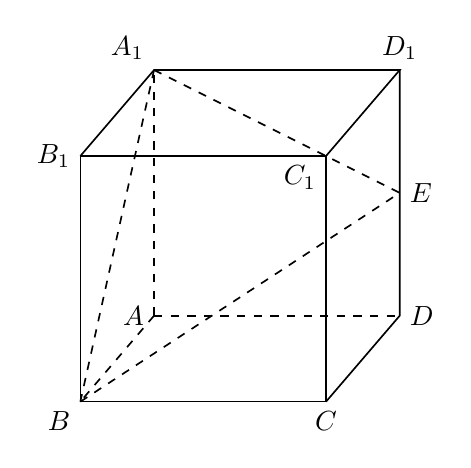
\begin{tikzpicture}[scale=0.78, semithick]
  \coordinate (B)  at (0,0);
  \coordinate (C)  at (4,0);
  \coordinate (C1) at (4,4);
  \coordinate (B1) at (0,4);
  \coordinate (A)  at (1.2,1.4);
  \coordinate (D)  at (5.2,1.4);
  \coordinate (A1) at (1.2,5.4);
  \coordinate (D1) at (5.2,5.4);
  \coordinate (E)  at (5.2,3.4);

  % 可见棱
  \draw (B) -- (C) -- (C1) -- (B1) -- cycle;
  \draw (B1) -- (A1) -- (D1) -- (C1);
  \draw (D1) -- (D) -- (C);

  % 被遮挡的棱
  \draw[dashed] (A) -- (B);
  \draw[dashed] (A) -- (D);
  \draw[dashed] (A) -- (A1);

  % 辅助线：三角形 A1BE
  \draw[dashed] (A1) -- (B);
  \draw[dashed] (B) -- (E);
  \draw[dashed] (A1) -- (E);

  \node[below left]  at (B)  {$B$};
  \node[below]       at (C)  {$C$};
  \node[left]        at (B1) {$B_1$};
  \node[below left]  at (C1) {$C_1$};
  \node[above left]  at (A1) {$A_1$};
  \node[above]       at (D1) {$D_1$};
  \node[left]        at (A)  {$A$};
  \node[right]       at (D)  {$D$};
  \node[right]       at (E)  {$E$};
\end{tikzpicture}
\end{center}
\nopagebreak[4]
\Needspace{4\baselineskip}
\textbf{解析}
\Needspace{5\baselineskip}
设正方体棱长为 $2$，建立空间直角坐标系：以 $A$ 为原点，$\overrightarrow{AB}$、$\overrightarrow{AD}$、$\overrightarrow{AA_1}$ 分别为 $x$、$y$、$z$ 轴正方向。则
\nopagebreak[4]
\[A(0,0,0),\ B(2,0,0),\ D(0,2,0),\ A_1(0,0,2),\ B_1(2,0,2),\ C_1(2,2,2),\ D_1(0,2,2).\]
因 $E$ 是 $DD_1$ 的中点，故 $E(0,2,1)$。
\Needspace{5\baselineskip}
（1）平面 $ABB_1A_1$ 即 $y=0$ 平面，其法向量可取 $\boldsymbol n=(0,1,0)$。又
\nopagebreak[4]
\[\overrightarrow{BE}=(-2,2,1),\qquad |\overrightarrow{BE}|=\sqrt{4+4+1}=3.\]
\Needspace{5\baselineskip}
设直线 $BE$ 与平面 $ABB_1A_1$ 所成的角为 $\theta$，则
\nopagebreak[4]
\[\sin\theta=\frac{|\overrightarrow{BE}\cdot\boldsymbol n|}{|\overrightarrow{BE}||\boldsymbol n|}
=\frac{2}{3}.\]
（2）存在，$F$ 为棱 $C_1D_1$ 的中点。证明如下。
\Needspace{5\baselineskip}
设 $F(t,2,2)$（$0\leqslant t\leqslant2$），则
\nopagebreak[4]
\[\overrightarrow{B_1F}=(t-2,2,0).\]
\Needspace{5\baselineskip}
平面 $A_1BE$ 中，
\nopagebreak[4]
\[\overrightarrow{A_1B}=(2,0,-2),\qquad\overrightarrow{A_1E}=(0,2,-1),\]
\Needspace{5\baselineskip}
其法向量
\nopagebreak[4]
\[\boldsymbol m=\overrightarrow{A_1B}\times\overrightarrow{A_1E}=(4,2,4),\]
\Needspace{5\baselineskip}
可取 $\boldsymbol m=(2,1,2)$。于是
\nopagebreak[4]
\[B_1F\parallel\text{\text{平面} }A_1BE\iff\overrightarrow{B_1F}\cdot\boldsymbol m=0
\iff2(t-2)+2=0\iff t=1.\]
\Needspace{5\baselineskip}
即 $F$ 为 $C_1D_1$ 的中点。此时平面 $A_1BE$ 的方程为 $2x+y+2z=4$，而
\nopagebreak[4]
\[2\cdot2+0+2\cdot2=8\neq4,\]
故 $B_1\notin$ 平面 $A_1BE$，从而 $B_1F\parallel$ 平面 $A_1BE$（而非在其内）。由 $t=1$ 唯一，这样的点 $F$ 唯一存在。

\gkanswer{答案：（1）$\dfrac23$；（2）存在，$F$ 为棱 $C_1D_1$ 的中点。}

\end{answer}
\begin{answer}
\gksolhead{19}{}

\textbf{题目}：

为了考察冰川的融化状况，一支科考队在某冰川上相距 $8$ km 的 $A$，$B$ 两点各建一个考察基地。视冰川面为平面形，以过 $A$，$B$ 两点的直线为 $x$ 轴，线段 $AB$ 的垂直平分线为 $y$ 轴建立平面直角坐标系（如图）。在直线 $x=2$ 的右侧，考察范围为到点 $B$ 的距离不超过 $\dfrac{6\sqrt5}{5}$ km 的区域；在直线 $x=2$ 的左侧，考察范围为到 $A$，$B$ 两点的距离之和不超过 $4\sqrt5$ km 的区域。

（1）求考察区域边界曲线的方程；

（2）如图所示，设线段 $P_1P_2$，$P_2P_3$ 是冰川的部分边界线（不考虑其他边界），当冰川融化时，边界线沿与其垂直的方向朝考察区域平行移动，第一年移动 $0.2$ km，以后每年移动的距离为前一年的 $2$ 倍。求冰川边界线移动到考察区域所需的最短时间。
\nopagebreak[4]
\begin{center}% 2010 年湖南卷理科第 19 题：冰川边界与考察区域的平面示意图。
% 来源 PDF：普通高考/2010/2010湖南理.pdf，SHA-256 db6274a80ebb0022ff1b91b2cd3714fe8cca335e48be69805dcd87cdefd8c8d1。
% 原页：第 2 页（A3 三栏）第 1 栏下部，书页码 602。
% 重绘依据：照原页坐标系，A(-4,0)、B(4,0)，冰界线 P1P2（斜线）与 P2P3（水平线），
%   P1(-5√3,-1)、P2(-8√3/3,6)、P3(8,6)；虚线 x=2 为左右两种考察范围的分界；
%   「已融化」「冰川」分列斜界线两侧，「区域」标于 x=2 右侧。
\begin{tikzpicture}[scale=0.62, semithick]
  \draw[->] (-9.8,0) -- (9.8,0) node[right] {$x$};
  \draw[->] (0,-2.6) -- (0,7.7) node[above] {$y$};

  \coordinate (A)  at (-4,0);
  \coordinate (B)  at (4,0);
  \coordinate (P1) at (-8.660,-1);
  \coordinate (P2) at (-4.619,6);
  \coordinate (P3) at (8,6);

  \draw (P1) -- (P2) -- (P3);
  \draw[dashed] (2,-2.4) -- (2,7.5);

  \fill (A) circle (1.2pt);
  \fill (B) circle (1.2pt);
  \fill (P1) circle (1.2pt);
  \fill (P2) circle (1.2pt);
  \fill (P3) circle (1.2pt);

  \node[below left]  at (A)  {$A(-4,0)$};
  \node[below right] at (B)  {$B(4,0)$};
  \node[below left]  at (P1) {$P_1(-5\sqrt3,-1)$};
  \node[left]        at (P2) {$P_2\left(-\dfrac{8\sqrt3}{3},6\right)$};
  \node[right]       at (P3) {$P_3(8,6)$};
  \node[below left]  at (0,0) {$O$};

  \node[below] at (2,-2.45) {$x=2$};

  % 冰川、已融化（沿界线两侧，照原页字位）
  \node at (-7.3,1.9) {已};
  \node at (-6.9,3.1) {融};
  \node at (-6.5,4.3) {化};
  \node at (-1.2,2.2) {冰};
  \node at (6.6,1.4) {川};

  \node at (3.3,6.55) {区域};
\end{tikzpicture}
\end{center}
\nopagebreak[4]
\Needspace{4\baselineskip}
\textbf{解析}
由 $|AB|=8$ 及坐标系建法，$A(-4,0)$，$B(4,0)$。
\Needspace{5\baselineskip}
（1）在直线 $x=2$ 的右侧，考察区域是以 $B(4,0)$ 为圆心、半径 $\dfrac{6\sqrt5}{5}$ 的圆面在该侧的部分，边界为
\nopagebreak[4]
\[(x-4)^2+y^2=\frac{36}{5}\qquad(x\geqslant2).\]
\Needspace{5\baselineskip}
在直线 $x=2$ 的左侧，考察区域是以 $A$、$B$ 为焦点、长轴长 $2a=4\sqrt5$ 的椭圆面在该侧的部分。此时 $a=2\sqrt5$，$c=4$，
\nopagebreak[4]
\[b^2=a^2-c^2=20-16=4,\]
\Needspace{5\baselineskip}
边界为
\nopagebreak[4]
\[\frac{x^2}{20}+\frac{y^2}{4}=1\qquad(x\leqslant2).\]
两段曲线在 $x=2$ 处相接：代入分别得 $y^2=\dfrac{36}{5}-4=\dfrac{16}{5}$ 与 $y^2=4\left(1-\dfrac4{20}\right)=\dfrac{16}{5}$，交点为 $\left(2,\pm\dfrac{4\sqrt5}{5}\right)$，故边界曲线为上述两段弧的并。
\Needspace{5\baselineskip}
（2）直线 $P_1P_2$ 过 $P_1(-5\sqrt3,-1)$、$P_2\left(-\dfrac{8\sqrt3}{3},6\right)$，斜率
\nopagebreak[4]
\[k=\frac{6-(-1)}{-\dfrac{8\sqrt3}{3}+5\sqrt3}=\frac{7}{\dfrac{7\sqrt3}{3}}=\sqrt3,\]
\Needspace{5\baselineskip}
故其方程为
\nopagebreak[4]
\[\sqrt3x-y+14=0.\]
\Needspace{5\baselineskip}
考察区域在直线 $P_1P_2$ 的右下方。对椭圆 $\dfrac{x^2}{20}+\dfrac{y^2}{4}=1$，函数 $\sqrt3x-y$ 的最小值为
\nopagebreak[4]
\[-\sqrt{20\cdot3+4\cdot1}=-8,\]
\Needspace{5\baselineskip}
在点 $\left(-\dfrac{5\sqrt3}{2},\dfrac12\right)$ 处取得（该点 $x<2$，属左段边界）。故区域上
\nopagebreak[4]
\[\sqrt3x-y+14\geqslant14-8=6,\]
\Needspace{5\baselineskip}
直线 $P_1P_2$ 到考察区域的（垂直）距离为
\nopagebreak[4]
\[d_1=\frac{6}{\sqrt{3+1}}=3,\]
且该最近点处的垂足 $\left(-4\sqrt3,2\right)$ 落在线段 $P_1P_2$ 上（其横坐标介于 $-5\sqrt3$ 与 $-\dfrac{8\sqrt3}{3}$ 之间）。
\Needspace{5\baselineskip}
直线 $P_2P_3$ 为 $y=6$。区域内点的纵坐标的最大值为 $\dfrac{6\sqrt5}{5}$（在圆的上顶点 $\left(4,\dfrac{6\sqrt5}{5}\right)$ 处取得，$\dfrac{6\sqrt5}{5}>2$），故
\nopagebreak[4]
\[d_2=6-\frac{6\sqrt5}{5}=\frac{30-6\sqrt5}{5}\approx3.32>3.\]
故边界线到考察区域的最短距离为 $3$ km，由 $P_1P_2$ 段达到。
\Needspace{5\baselineskip}
设第 $n$ 年末累计移动 $s_n$ km，则
\nopagebreak[4]
\[s_n=0.2(1+2+\cdots+2^{n-1})=0.2(2^n-1).\]
\Needspace{5\baselineskip}
令 $s_n\geqslant3$：
\nopagebreak[4]
\[0.2(2^n-1)\geqslant3\iff2^n\geqslant16\iff n\geqslant4.\]
故恰好 $4$ 年时累计移动 $0.2\times15=3$ km，边界线到达考察区域；$3$ 年时累计 $1.4$ km，尚差 $1.6$ km。所求最短时间为 $4$ 年。

\gkanswer{答案：（1）$(x-4)^2+y^2=\dfrac{36}{5}$（$x\geqslant2$）与 $\dfrac{x^2}{20}+\dfrac{y^2}{4}=1$（$x\leqslant2$）；（2）$4$ 年。}

\end{answer}
\begin{answer}
\gksolhead{20}{}

\textbf{题目}：

已知函数 $f(x)=x^2+bx+c$（$b$，$c\in\mathbf R$），对任意的 $x\in\mathbf R$，恒有 $f'(x)\leqslant f(x)$。

（1）证明：当 $x\geqslant0$ 时，$f(x)\leqslant(x+c)^2$；

（2）若对满足题设条件的任意 $b$，$c$，不等式 $f(c)-f(b)\leqslant M(c^2-b^2)$ 恒成立，求 $M$ 的最小值。

\Needspace{4\baselineskip}
\textbf{解析}
\Needspace{5\baselineskip}
由 $f'(x)=2x+b$，题设 $f'(x)\leqslant f(x)$ 即
\nopagebreak[4]
\[x^2+(b-2)x+(c-b)\geqslant0\quad(\forall x\in\mathbf R).\]
\Needspace{5\baselineskip}
故判别式
\nopagebreak[4]
\[\Delta=(b-2)^2-4(c-b)=b^2+4-4c\leqslant0\iff c\geqslant\frac{b^2+4}{4}.\]
特别地 $c\geqslant1$。
\Needspace{5\baselineskip}
（1）当 $x\geqslant0$ 时，
\nopagebreak[4]
\[(x+c)^2-f(x)=x^2+2cx+c^2-(x^2+bx+c)=(2c-b)x+c(c-1).\]
\Needspace{5\baselineskip}
因 $c\geqslant1$，故 $c(c-1)\geqslant0$。又
\nopagebreak[4]
\[2c\geqslant\frac{b^2+4}{2}.\]
\Needspace{5\baselineskip}
当 $b\leqslant0$ 时 $2c-b>0$；当 $b>0$ 时
\nopagebreak[4]
\[2c-b\geqslant\frac{b^2+4}{2}-b=\frac{(b-1)^2+3}{2}>0.\]
\Needspace{5\baselineskip}
故 $2c-b>0$ 恒成立。于是 $x\geqslant0$ 时 $(2c-b)x\geqslant0$，从而
\nopagebreak[4]
\[(x+c)^2-f(x)\geqslant0\iff f(x)\leqslant(x+c)^2.\]
\Needspace{5\baselineskip}
（2）对任意满足条件的 $b$，$c$，
\nopagebreak[4]
\[f(c)-f(b)=(c^2+bc+c)-(2b^2+c)=c^2+bc-2b^2.\]
\Needspace{5\baselineskip}
注意到
\nopagebreak[4]
\[\frac32(c^2-b^2)-\bigl(c^2+bc-2b^2\bigr)
=\frac{3c^2-3b^2-2c^2-2bc+4b^2}{2}
=\frac{(c-b)^2}{2}\geqslant0,\]
故 $M=\dfrac32$ 时不等式对任意 $b$，$c$ 恒成立。
\Needspace{5\baselineskip}
再证 $M$ 不能更小。取
\nopagebreak[4]
\[c=2,\qquad b=2-\varepsilon\quad\left(0<\varepsilon<\frac14\right),\]
\Needspace{5\baselineskip}
则
\nopagebreak[4]
\[\frac{b^2+4}{4}=\frac{(2-\varepsilon)^2+4}{4}=2-\varepsilon+\frac{\varepsilon^2}{4}\leqslant2=c,\]
\Needspace{5\baselineskip}
即该 $(b,c)$ 满足题设条件。此时
\nopagebreak[4]
\[c^2-b^2=4\varepsilon-\varepsilon^2>0,\]
\nopagebreak[4]
\[f(c)-f(b)=6\varepsilon-2\varepsilon^2,\]
\nopagebreak[4]
\[\frac{f(c)-f(b)}{c^2-b^2}=\frac{6-2\varepsilon}{4-\varepsilon}\longrightarrow\frac32\quad(\varepsilon\to0^+).\]
\Needspace{5\baselineskip}
故对任何 $M<\dfrac32$，取 $\varepsilon$ 充分小即有不等式不成立。所以 $M$ 的最小值为
\nopagebreak[4]
\[M_{\min}=\frac32.\]

\gkanswer{答案：（1）证明见解析；（2）$\dfrac32$。}

\end{answer}
\begin{answer}
\gksolhead{21}{}

\textbf{题目}：

数列 $\{a_n\}$（$n\in\mathbf N^*$）中，$a_1=a$，$a_{n+1}$ 是函数 $f_n(x)=\dfrac13x^3-\dfrac12(3a_n+n^2)x^2+3n^2a_nx$ 的极小值点。

（1）当 $a=0$ 时，求通项 $a_n$；

（2）是否存在 $a$，使数列 $\{a_n\}$ 是等比数列？若存在，求 $a$ 的取值范围；若不存在，请说明理由。

\Needspace{4\baselineskip}
\textbf{解析}
\Needspace{5\baselineskip}
对
\nopagebreak[4]
\[f_n(x)=\frac13x^3-\frac12(3a_n+n^2)x^2+3n^2a_nx\]
\Needspace{5\baselineskip}
求导：
\nopagebreak[4]
\[f_n'(x)=x^2-(3a_n+n^2)x+3n^2a_n=(x-3a_n)(x-n^2).\]
\Needspace{5\baselineskip}
故驻点为 $x=3a_n$ 与 $x=n^2$。又
\nopagebreak[4]
\[f_n''(x)=2x-(3a_n+n^2),\]
\Needspace{5\baselineskip}
在较大驻点处 $f_n''>0$，在较小驻点处 $f_n''<0$，故极小值点为较大的驻点，即
\nopagebreak[4]
\[a_{n+1}=\max\{3a_n,n^2\}.\]
\Needspace{5\baselineskip}
（1）当 $a=0$ 时，
\nopagebreak[4]
\[a_1=0,\quad a_2=\max\{0,1\}=1,\quad a_3=\max\{3,4\}=4.\]
\Needspace{5\baselineskip}
当 $n\geqslant3$ 时，若 $a_n=4\cdot3^{n-3}$，则
\nopagebreak[4]
\[3a_n=4\cdot3^{n-2}>n^2\quad(n\geqslant4),\]
\Needspace{5\baselineskip}
故 $a_{n+1}=3a_n$。于是
\nopagebreak[4]
\[a_n=\begin{cases}0,&n=1,\\[2pt]1,&n=2,\\[2pt]4\cdot3^{n-3},&n\geqslant3.\end{cases}\]
（2）存在，$a$ 的取值范围为 $a>\dfrac49$。
\Needspace{5\baselineskip}
因 $a_2=\max\{3a,1\}\geqslant1>0$，故 $n\geqslant2$ 时 $a_n>0$。又
\nopagebreak[4]
\[a_{n+1}=\max\{3a_n,n^2\}\geqslant3a_n.\]
\Needspace{5\baselineskip}
若 $\{a_n\}$ 是公比为 $q$ 的等比数列，则对 $n\geqslant2$
\nopagebreak[4]
\[q=\frac{a_{n+1}}{a_n}\geqslant3.\]
若 $q>3$，则对每个 $n$ 都有 $q a_n>3a_n$，故 $a_{n+1}=n^2$，从而 $a_n=(n-1)^2$（$n\geqslant2$），其相邻项之比 $\dfrac{n^2}{(n-1)^2}$ 不是常数，矛盾。故只能 $q=3$。
\Needspace{5\baselineskip}
于是对一切 $n\in\mathbf N^*$ 必须有 $a_{n+1}=3a_n$（且 $3a_n>n^2$，否则 $3a_n=n^2$ 时 $f_n'$ 有重根、无极小值点）。由 $a_1=a$ 得
\nopagebreak[4]
\[a_n=3^{n-1}a,\]
\Needspace{5\baselineskip}
条件 $3a_n>n^2$ 即
\nopagebreak[4]
\[3^n a>n^2\quad(\forall n\in\mathbf N^*)\iff a>\frac{n^2}{3^n}\quad(\forall n\in\mathbf N^*).\]
\Needspace{5\baselineskip}
而 $\dfrac{n^2}{3^n}$ 在 $n=2$ 时取最大值 $\dfrac49$（$n=1$ 为 $\dfrac13$，$n=3$ 为 $\dfrac13$，$n\geqslant4$ 递减），故
\nopagebreak[4]
\[a>\frac49.\]
反之，$a>\dfrac49$ 时对一切 $n$ 有 $3^n a>n^2$，从而 $a_{n+1}=3a_n$，$\{a_n\}$ 是公比为 $3$ 的等比数列。
故存在，且 $a$ 的取值范围为 $\left(\dfrac49,+\infty\right)$。

\gkanswer{答案：（1）$a_1=0$，$a_2=1$，$a_n=4\cdot3^{n-3}$（$n\geqslant3$）；（2）存在，$a>\dfrac49$。}

\end{answer}